\subsection{Giao diện kết quả bảng khảo sát}

\begin{figure}[H]
    \centering
    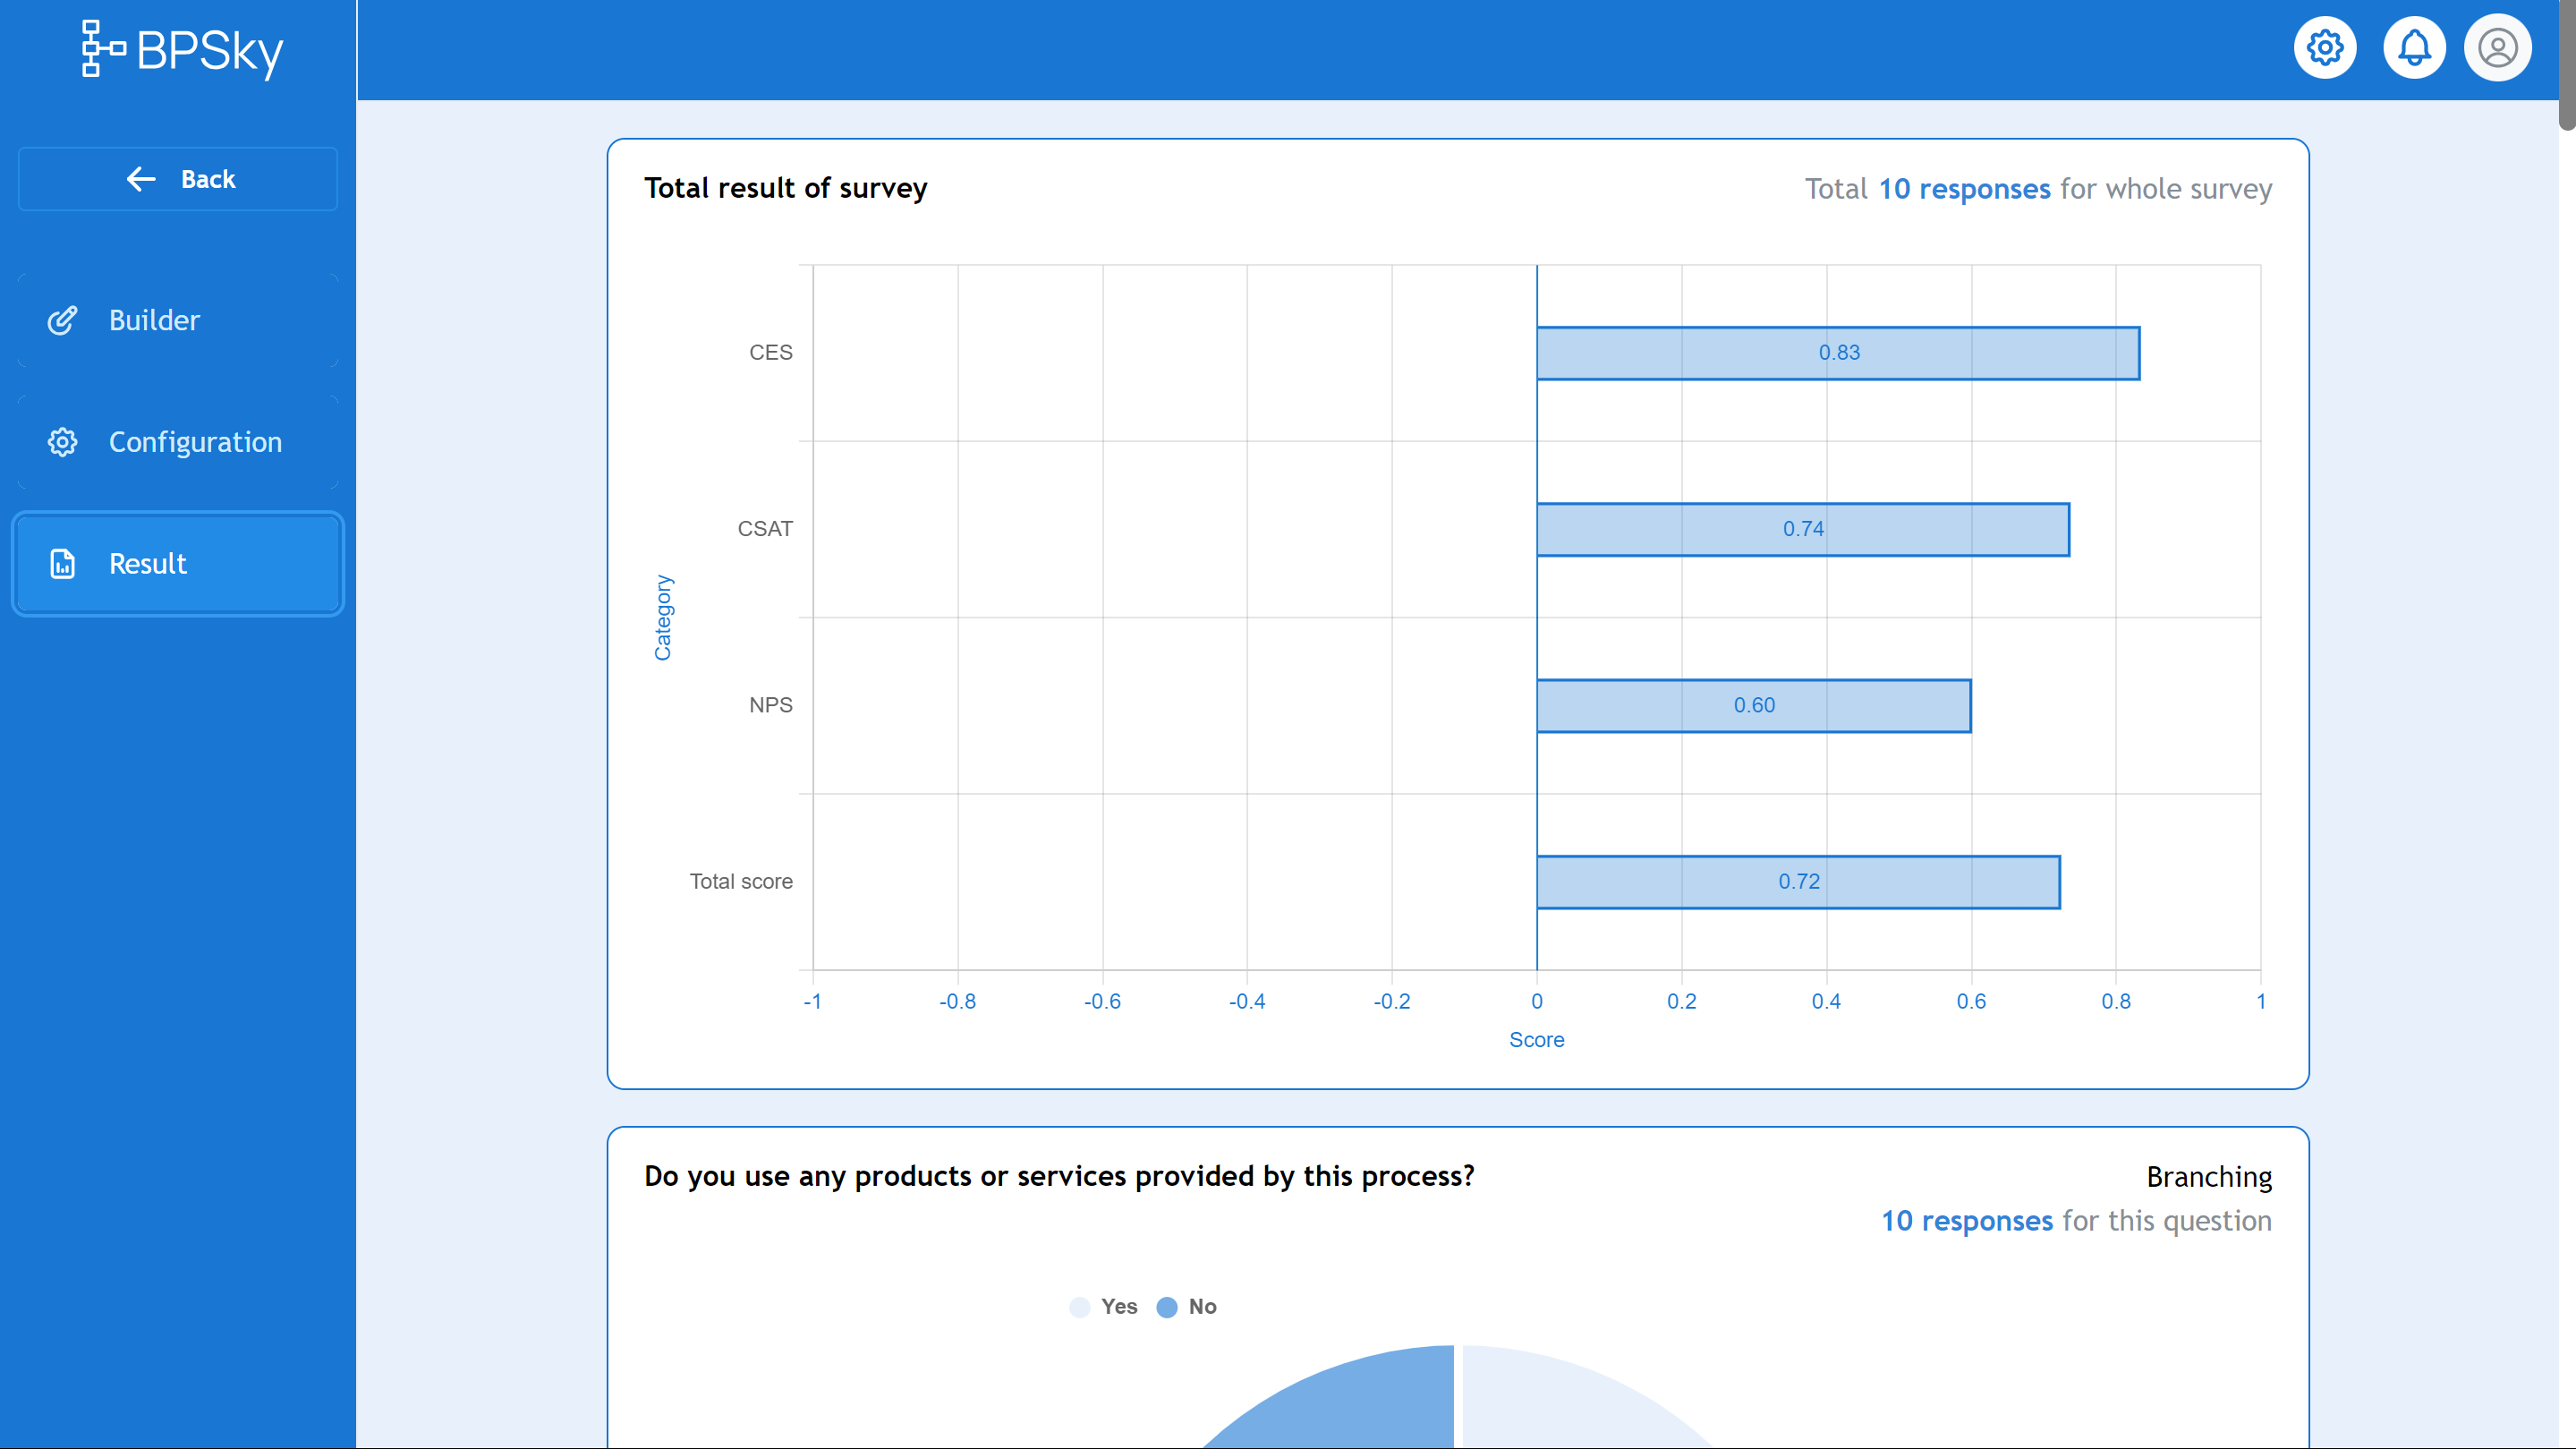
\includegraphics[ width = \linewidth]{Content/Hiện thực hệ thống/documents/Hiện thực giao diện người dùng/images/SurveyResult.png}
    \vspace{0.5cm}
    \caption{Giao diện kết quả bảng khảo sát}
    \label{fig: Giao diện kết quả bảng khảo sát}
\end{figure}

Sau khi người dùng chọn biểu tượng kết quả trên thanh công cụ thì hệ thống sẽ chuyển hướng người dùng tới trang giao diện kết quả bảng khảo sát. Giao diện này bao gồm kết quả thống kê chi tiết lựa chọn của từng câu hỏi trong bảng khảo sát và kết quả tổng hợp của bảng khảo sát. Tùy thuộc vào loại câu hỏi mà sẽ được thể hiện thông qua biểu đồ khác nhau:
\begin{itemize}
    \item Loại câu hỏi rẽ nhánh - Branching: Sử dụng biểu đồ tròn để thể hiện phần trăm số lượng câu trả lời cho từng lựa chọn Có/Không.
    \item Loại câu hỏi Multiple choice/CES/CSAT/NPS: Sử dụng biểu đồ cột để thể hiện phần trăm số lượng câu trả lời cho từng lựa chọn. Bao gồm có 7 lựa chọn (tương ứng từ 1 đến 7) đối với loại câu hỏi CES và CSAT, và 10 lựa chọn (tương ứng từ 0 đến 10) đối với loại câu hỏi NPS.
    \item Loại câu hỏi CES-IN/CSAT-IN: Sử dụng dạng danh sách câu trả lời ngắn để liệt kê những ý kiến của người làm khảo sát.
\end{itemize}